\documentclass[12pt, letterpaper]{article}
\usepackage[T1]{fontenc}
\usepackage[italian]{babel}
\usepackage{hyphenat}
\hyphenation{mate-mati-ca recu-perare}
\usepackage{graphicx}

\title{Relazione per il Progetto del Corso di Programmazione e Modellazione ad Oggetti}
\author{Elia Renzoni, Annarosa Clemente, Eloi Ricci, Giuseppe Benedetti}
\date{25/05/2024}

\begin{document}

\begin{figure}
    \centering
    
\includegraphics[width=0.5\linewidth]{logo-uni.png}
\end{figure}

\maketitle

\newpage
\tableofcontents
\newpage
\section{Analisi}
    \subsection{Analisi dei Requisiti}
        \textbf{Labirinto} è un gioco a singolo utente multi-livello in cui il giocatore deve uscire dal  labirinto in cui è intrappolato.
        La mappa in cui si muove è delimitata da mura ed è cosparsa di ostacoli (quali bombe, NPC e bucce di banana) e premi (come le casse contenenti monete e l'incantesimo di immunità). 
        \\
        Il giocatore deve raccogliere più monete possibili in un tempo ragionevole; al termine della partita questi due valori concorreranno alla creazione di una classifica nella quale saranno visibili i record ottenuti dalle varie partite. 
        \\
        Il giocatore potrà personalizzare il suo game-play scegliendo un nome utente, un livello di difficoltà tra EASY, NORMAL e HARD e il personaggio con cui giocare; i personaggi sono due, un ragazzo e una ragazza: Linda e Fonzie.
        \\
        All'aumentare del livello di difficoltà aumenta anche il numero di ostacoli.
        \newpage
    \subsection{Lista dei Requisiti:}
        \textbf{Requisiti funzionali:}
            \begin{itemize}
                \item Implementazione degli ostacoli:
                \begin{itemize}
                    \item Bomba: se colpita fa perdere delle  monete al giocatore. Il numero di monete perse dipende dal livello di difficoltà della partita.
                    \item NPC: se toccati uccidono il personaggio, terminando così la partita.
                    \item Banana: se presa fa retrocedere il personaggio di cinque posizioni nel caso di Fonzie, altrimenti di sette posizioni nel caso di Linda.
                \end{itemize}
                \item Implementazione dei premi:
                \begin{itemize}
                    \item Incantesimo di immunità: se preso rende immune il personaggio. L'effetto avrà durata non oltre i successivi tre spostamenti effettuati dal giocatore.
                    \item Cassa: contiene delle monete il cui numero dipende dal livello di difficoltà della partita. Se colpita il giocatore riscuote le monete contenute.
                \end{itemize}
                \item Implementazione delle mura: bloccano il passaggio del giocatore.
                \item Implementazione dei personaggi:
                \begin{itemize}
                    \item Linda: la più veloce, ogni movimento la fa spostare di due posizioni nella mappa.
                    \item Fonzie: ha una vita extra, muore la seconda volta che colpisce un NPC.
                \end{itemize}
                \item Il programma deve permette di eseguire i movimenti dell'utente. 
                \item Il programma deve permette all'utente di scegliere un nome, un personaggio e una modalità di gioco.
                \item A fine partita deve essere visualizzata una classifica delle dieci migliori partite, ordinata in base al minor tempo impiegato per uscire dal labirinto e al maggior numero di monete ottenute.
                \item Il programma deve creare dinamicamente e casualmente la mappa.
                \item La partita va gestita applicando le regole descritte qui sopra.
            \end{itemize}
        \textbf{Requisiti non funzionali:}
            \begin{itemize}
                \item Gestione dei suoni.
                \item Ottimizzazione delle texture fatta tramite l'ausilio della bufferizzazione delle immagini.
                \item Gestione e salvataggio dei dati di gioco su un file.
            \end{itemize}
    \subsection{Modello del Dominio}
        Labirinto deve organizzare il gioco in base al livello di difficoltà selezionato, questo è rappresentato dall'entità \textbf{GameDifficult}, la quale determina il numero e tipo di oggetti  -  premi e ostacoli - che popoleranno la mappa. Gli oggetti sono rappresentati dall'entità \textbf{Element}.\\
        I principali attori coinvolti in una partita sono:
        \begin{itemize}
            \item  L'utente, rappresentato dall’entità \textbf{IUser}, la quale permette di impostare un nome utente.
            \item Il personaggio, rappresentato dall'entità \textbf{Player} la quale contiene le caratteristiche principali dei personaggi, come il nome (Linda o Fonzie), la velocità e la vita.
            \item La mappa, rappresentata dall’entità \textbf{IGameMap}, che deve essere generata in base al livello di difficoltà scelto. 
            \item  Il risultato finale rappresentato dall'entità \textbf{IResult}. Questa crea un record in cui il nome del giocatore è associato al personaggio scelto, alle monete raccolte e al tempo impiegato.
            \item La classifica, rappresentata dall'entità \textbf{IRanking}, la quale aggiunge i record dei giocatori in un file e li ordina in base al tempo impiegato e alle monete ottenute.
            \item Il movimento del personaggio, gestito dall'entità \textbf{Movement}, la quale gli consente di muoversi attraverso la mappa, lo blocca quando incontra delle mura, modifica la sua posizione se inciampa su una banana e controlla per quanto tempo l'incantesimo immunità avrà ancora effetto.
        \end{itemize}
        \begin{figure}
            \centering
            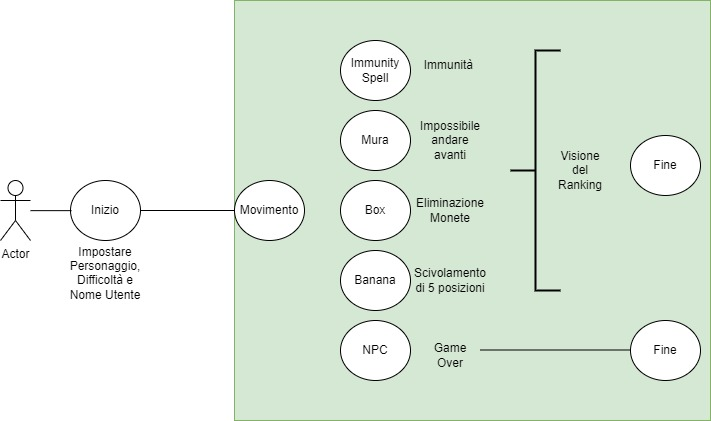
\includegraphics[width=1\linewidth]{user_case.jpg}
            \caption{Diagramma d'uso}
        \end{figure}
        \begin{figure}
            \centering
            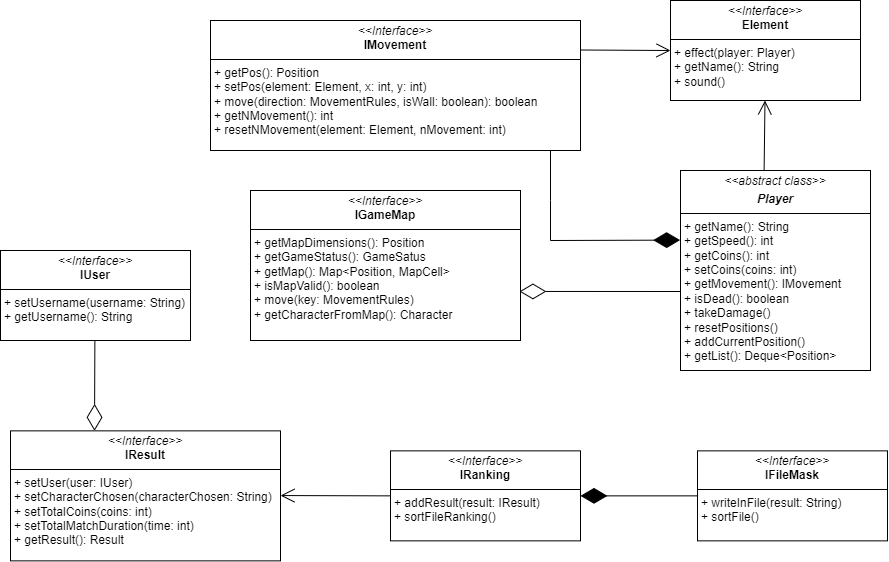
\includegraphics[width=1\linewidth]{model_domain.png}
            \caption{Modello del dominio}
        \end{figure}
        La \textbf{figura 1} mostra i casi d'uso del software. Ogni partita inizia con l'inserimento del proprio nome utente, la selezione del personaggio e del livello di difficoltà. Una volta avviata la partita il giocatore dovrà muoversi nella mappa. L'incontro con i vari ostacoli e premi modifica l'esito del gioco. A fine partita, il risultato dell'utente è salvato nella classifica e ne vengono mostrati i migliori dieci risultati se, invece, l'utente incontra un NPC, il gioco termina mostrando la schermata di Game-Over e il suo risultato, mentre la classifica non viene stampata.
        \\
        \\
        La \textbf{figura 2} mostra il modello del dominio rappresentato con le interfacce e una classe astratta. Si possono vedere fin da subito le relazioni tra le diverse entità: le più importanti sono quelle di aggregazione e composizione che riguardano le entità \textbf{Player}, \textbf{IGameMap}, \textbf{IResult} e \textbf{IRanking}; è presente anche la relazione di utilizzo.
    \newpage
\section{Design}
    \subsection{Architettura}
        L'architettura del software si basa sul pattern MVC (Model - View - Controller).
        Il Controller funge da disacoppiatore, in quanto elimina ogni interazione diretta tra Model e View passando i riferimenti del primo alla View e utilizzando i metodi pubblici delle entità del modello per modificare i dati a fronte di ogni evento generato dal viewer.\\
        Inoltre, abbiamo integrato il  pattern Observer, secondo cui ci sono dei generatori di eventi e degli osservatori di quest'ultimi: i primi si trovano nella view, mentre i secondi sono nel modello e vengono attivati dal controller, il quale fa da intermediario.
    \newpage
    \subsection{Design Dettagliato}
        In questa sezione abbiamo riportato i diagrammi UML con le relative descrizioni delle entità che rappresentano le macro componenti del nostro progetto. \\
        Oltre all'impostazione architetturale del software secondo i pattern MVC e Observer, abbiamo utilizzato il design pattern creazionale \textbf{Singleton} laddove non era necessario avere più istanze della stessa entità. Per realizzarlo abbiamo reso privato il costruttore e abbiamo aggiunto un metodo statico e pubblico che lo chiama restituendo la nuova, o la precedente, istanza dell'entità.\\ 
        Le entità che utilizzano il design pattern Singleton sono le seguenti:
        \begin{itemize}
            \item Controller, appartenente al controller.
            \item Fonzie, appartenente al modello.
            \item Linda, appartenente al modello.
            \item FileMask, appartenente al modello.
            \item Ranking, appartenente al modello.
            \item Result, appartenente al modello.
            \item User, appartenente al modello.
            \item GameOverFrame, appartenente alla view.
            \item InputPlayer, appartenente alla view.
            \item MatrixPrinter, appartenente alla view.
        \end{itemize}
        Abbiamo inoltre deciso di utilizzare il pattern comportamentale \textbf{Template Method} che consente alle entità Fonzie e Linda di unificare l'effetto della banana rispetto al loro personaggio.
    \newpage
    \subsection{Design del Modello}
        \subsubsection{Gestione delle Posizioni e del Movimento}
            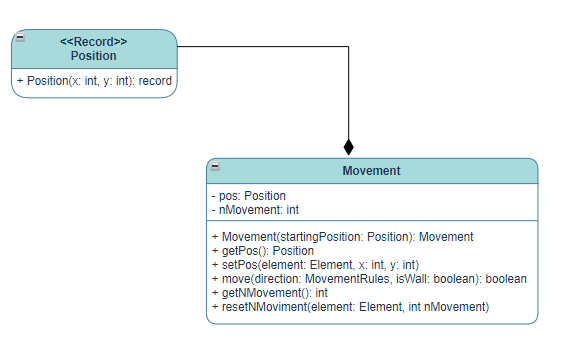
\includegraphics[width=1\textwidth]{moviment_position.png}\\
            \textbf{Problema}\\ \\
            Una parte fondamentale del gioco è il movimento.
            L'implementazione deve tenere conto del fatto che se l'utente si trova nella posizione \verb|(x,y)|, allora un movimento in avanti o indietro deve produrre rispettivamente un incremento o un decremento del valore della coordinata \verb|row|. Viceversa, ogni spostamento verso sinistra o destra deve comportare rispettivamente un incremento o un decremento del valore della coordinata \verb|column|.\\ \\
            \textbf{Soluzione}\\ \\
            Date le premesse nel problema, è stato necessario legare il movimento del personaggio alla struttura della mappa.
            Poiché questa si compone da un numero finito di celle identificabili con una coppia di coordinate, abbiamo scelto di sfruttarle per gestire lo spostamento. Questo va a modificare i valori delle coordinate attuali in base a dove l'utente intende spostarsi.
            Per implementare queste funzionalità abbiamo creato le entità \textbf{Position} e \textbf{Movement} che gestiscono rispettivamente le posizioni e il movimento. La prima rappresenta le due coordinate x e y che identificano la posizione del personaggio sulla mappa; la seconda è in relazione di aggregazione con Position in quanto viene inizialmente creata un'istanza di quest'ultima per impostare la posizione di partenza, che sarà poi modificata in seguito a ogni spostamento che il giocatore intende effettuare. Inoltre Movement fa uso dell'enumerato \textbf{MovementRules} che stabilisce le regole di movimento. Questa genera una coppia di coordinate da sommare a quelle attuali consentendo così lo spostamento. Se, ad esempio, sono in posizione \verb|row = 4| e \verb|column = 3|, in caso di spostamento a sinistra MovementRules restituisce la coppia (0, -1) che, sommata alla coppia di coordinate della posizione attuale, fa diminuire il valore di \verb|column| di 1.
            \\
            Movement è in relazione di composizione con l'entità \textbf{Player}, mentre Position è in relazione di composizione con \textbf{GameDifficulty} e di aggregazione con \textbf{GameMap}
        \subsubsection{Creazione del Personaggio}
            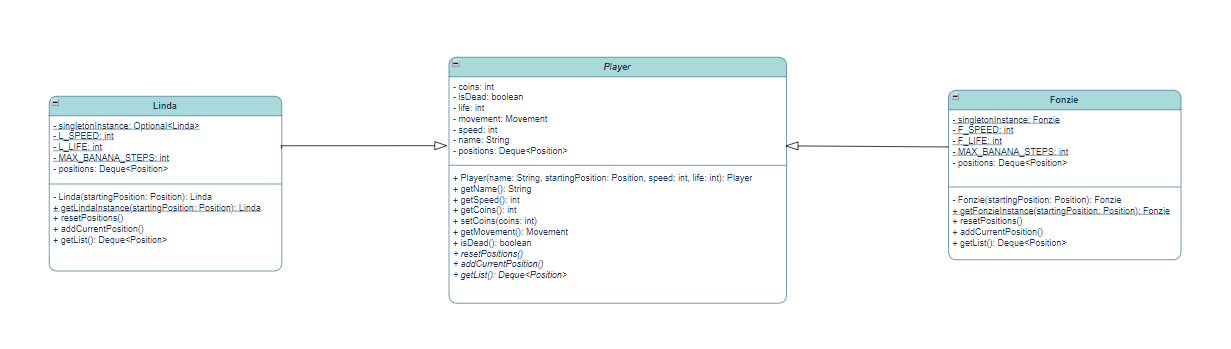
\includegraphics[width=1\textwidth]{player.png}
            \\
            \textbf{Problema}
            \\ \\
            L'utente gioca con un personaggio a scelta tra Linda e Fonzie. Le informazioni importanti da memorizzare legate al personaggio sono la vita (fondamentale in caso di uccisione da parte di un NPC), la velocità (che serve per impostare la lunghezza dei movimenti) e il numero di monete raccolte (utile per ottenere la posizione nel ranking). \\
            Un altro aspetto importante da gestire è dato dall'effetto dell'ostacolo banana, che fa retrocedere di cinque posizioni il giocatore, nel caso in cui venga usato il personaggio Fonzie, altrimenti lo fa retrocedere di sette posizioni.
            \\ \\
            \textbf{Soluzione}
            \\ \\
            % DA AGGIUNGERE LA MODIFICA AL METODO ASTRATTO
            Per implementare queste funzionalità abbiamo creato una classe astratta chiamata \textbf{Player}, che viene estesa dalle altre due rappresentanti i personaggi, quindi \textbf{Linda} e \textbf{Fonzie}. In questo modo si riducono le ripetizioni di codice dovute alle caratteristiche in comune tra i due personaggi, evitando così di violare il principio DRY.\\
            Per risolvere la questione legata all'effetto della banana, abbiamo deciso di memorizzare le ultime posizioni in cui il personaggio è andato. Per questo motivo, Player, oltre ai getter e i setter, espone i metodi astratti \verb|resetPosition()| e \verb|addCurrentPosition()|: il primo svuota la lista di posizioni dopo che è stata toccata la banana, mentre il secondo salva le posizioni occupate in una coda,  evitando che si ecceda la massima capacità prefissata, Da notare che l'effetto è attivato da altre entità, ma i metodi che permettono all'entità di subire l'effetto sono quelli sopra specificati (con l'aggiunta del metodo astratto \verb|getList()|) poiché riguardano il personaggio. I metodi astratti dell'entità Player sono implementati dalle entità Fonzie e Linda, in quanto devono personalizzarli rispetto al numero di passi indietro da effettuare. 
        \subsubsection{Gestione dei Risultati e del Ranking}
            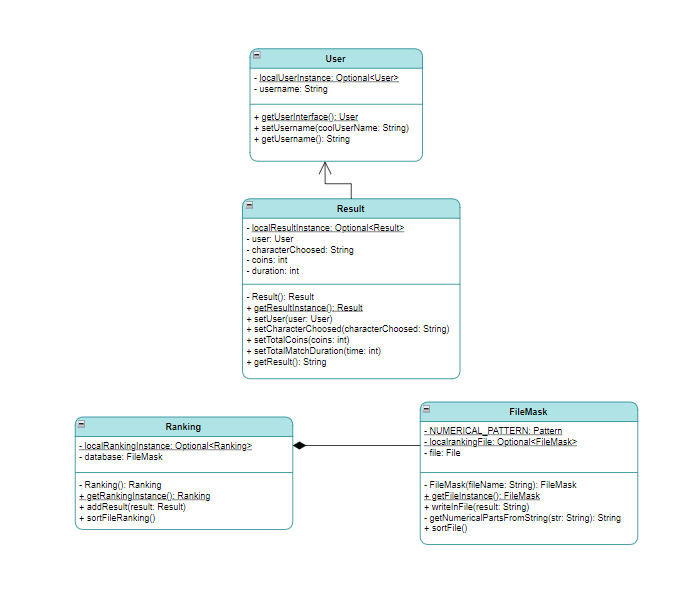
\includegraphics[width=\textwidth]{result_ranking.png}
            \textbf{Problema} 
            \\ \\
            In caso di vittoria, al termine di ogni partita l'utente deve poter visualizzare il proprio risultato e una classifica contente i dieci migliori risultati, mentre in caso di sconfitta deve poter vedere solo il proprio. %Una cosa molto importante per i risutalti è la loro formattazione, infatti è opportuno prendere i valori del gameplay dalle diverse entità, formattarle correttamente e poi memorizzarlo su un file, di cui si stampano solo le prime dieci posizioni più meritevoli\\ \\
            I risultati vanno salvati in un file a parte e ordinati in base al miglior tempo e numero di monetine (da qui devono essere presi i primi 10 da visualizzare in caso di vittoria)
            \\ \\
            \textbf{Soluzione} 
            \\ \\
            Per implementare queste funzionalità vengono modellate le entità \textbf{User}, \textbf{Result}, \textbf{Ranking} e \textbf{FileMask}. User deve memorizzare il nome scelto dall'utente, Result, invece, deve contenere il risultato della partita appena terminata. Quest'ultimo è composto dal nome dell'utente - per cui risulta utile associare la classe User a Result - il numero di monete raccolte e la durata del game-play. Una volta impostati i campi compone il risultato. 
            \\
            L'entità Ranking deve occuparsi di scrivere dentro il file contente la classifica e ordinarlo secondo il numero di monete ottenute e il tempo impiegato per terminare la partita. Queste attività di memorizzazione persistente e di ordinamento sono però affidate all'entità FileMask la quale consente la scrittura dei risultati su un file di testo e il loro ordinamento confrontandone i parametri riga per riga.
        \subsubsection{Creazione dei Premi e degli Ostacoli}
            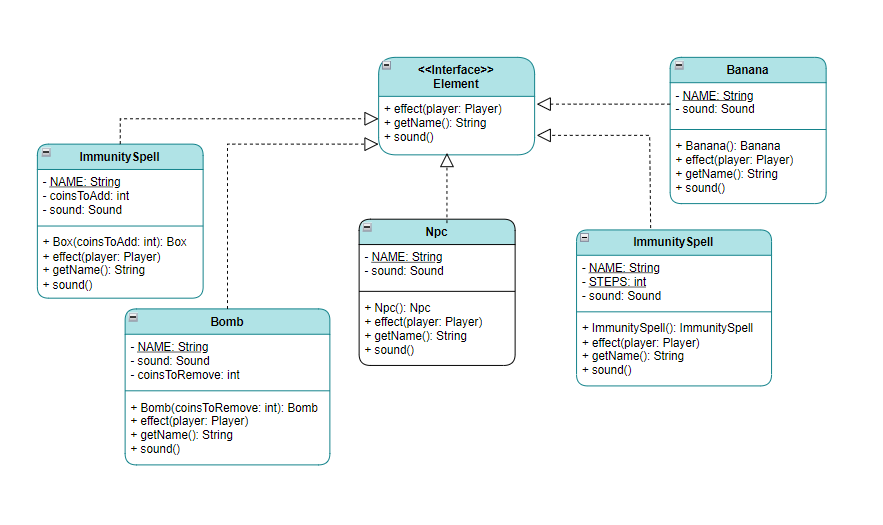
\includegraphics[width=\textwidth]{element.png}
            \\ \\ \\ \\ \\
            \textbf{Problema}
            \\ \\
            I premi e gli ostacoli sono le componenti principali del gioco poiché determinano il risultato finale della partita. I premi e gli ostacoli devono essere posizionati in modo randomico sulla mappa e in quantità differenti a seconda del livello di difficoltà selezionato. \\
            Le casse e gli incantesimi immunità una volta colpiti devono modificare lo stato del personaggio, le prime aggiungendo delle monete a quelle raccolte e i secondi una vita che rende immuni agli NPC. Gli ostacoli - NPC, banana e bomba - invece, devono modificare la vita del personaggio, la sua posizione e il numero di monete rispettivamente.
            \\ \\
            \textbf{Soluzione} 
            \\ \\
            I premi e gli ostacoli hanno un proprio effetto, nome e suono; queste informazioni sono gestite da appositi metodi che, essendo comuni a entrambi, sono stati incapsulati dentro l'interfaccia \textbf{Element}. Questa deve essere implementata dalle classi \textbf{Box}, \textbf{ImmunitySpell}, \textbf{NPC}, \textbf{Banana} e \textbf{Bomb}, le quali dovranno implementarne i metodi inserendo il corretto effetto, nome e suono. Ogni chiamata al metodo \verb|effect()| avrà una conseguenza sul personaggio, quindi il metodo avrà come parametro l'entità Player per poterne chiamare i metodi che ne modificano i campi.
            \\
            Inoltre, l'entità \textbf{Sound} si compone di tutte e cinque le entità sopra descritte.
            \\
        \subsubsection{Generazione della Mappa}
            \textbf{Problema} 
            \\ \\
            La generazione della mappa è una componente cruciale del progetto che gestisce la creazione dinamica della mappa di gioco e l'inserimento degli elementi al suo interno, garantendo la validità e coerenza della mappa stessa. 
            \\ \\
            \textbf{Soluzione} 
            \\ \\
            La classe responsabile di questo processo è \texttt{GameMap}, che segue i seguenti passaggi:
            \begin{itemize}
                \item \textbf{Creazione dei Valori di Generazione (\texttt{createsGenerationValues})}: All'interno del costruttore della classe \texttt{GameMap}, dopo aver inizializzato le dimensioni della mappa e il riferimento al personaggio, viene chiamato il metodo \texttt{createsGenerationValues} con un parametro di difficoltà. Questo metodo calcola il numero di punti disponibili sulla mappa, rimuovendo una certa quantità per garantire che ci sia almeno un percorso percorribile e non siano presenti solo muri. Successivamente inserisce questi valori in una mappa per la successiva generazione degli elementi.
                \item \textbf{Metodo \texttt{generateMap}}: La mappa viene generata in un ciclo \texttt{while} fino a che non viene considerata valida, provando un massimo di 30.000 generazioni. Alle iterazioni iniziali, vengono create le mura di confine. Successivamente, tutte le posizioni vuote vengono raccolte e gli elementi vengono inseriti sulla mappa basandosi sui valori precedentemente calcolati. Se durante la generazione si incontrano muri, questi vengono generati in coppia per formare una struttura coerente. Dopo aver popolato la mappa, viene inserito il punto di uscita ed eseguito un controllo di validità tramite \texttt{isMapValid}.
                \item \textbf{Valida la Mappa (\texttt{isMapValid})}: Questo metodo utilizza un approccio di ricerca basato su un insieme ordinato di posizioni da visitare, iniziando dalla posizione del personaggio. Per ogni posizione esaminata, vengono calcolate tutte le possibili posizioni raggiungibili e, se uno di questi percorsi può arrivare al punto di uscita, la mappa viene considerata valida.
            \end{itemize}
            Questo processo garantisce una mappa dinamica e coerente che supporta il gioco, mantenendo un equilibrio tra difficoltà e giocabilità.
    \subsection{Design del Controller}
        Il Controller è il componente che funge da intermediario tra il modello e la vista in un'architettura MVC. Nel nostro caso, il controller ha il compito di aggiornare le informazioni sulla partita a fronte di ogni movimento, modificare i dati del modello come il nome utente, il giocatore selezionato, il livello scelto e infine il risultato parziale che farà parte del ranking.
        \begin{itemize}
            \item \textbf{Problema}: Il Controller è formato da una sola classe che si occupa di mettere in comunicazione il modello con la vista. Il compito quindi è quello di memorizzare le due istanze e chiamare i rispettivi metodi a fronte di ogni evento generato dall'utente (gli eventi provengono dall'interfaccia grafica).
            \item \textbf{Soluzione}: La classe Controller sta principalmente in ascolto degli input generati dal giocatore. Questi sono dati dalla pressione dei tasti sulla tastiera e dalla scelta dei livelli e personaggi per avviare la partita. I principali metodi che implementano questa logica sono \texttt{getGameMap()}, \texttt{runGame()} e \texttt{getData()}. Il primo si occupa di ascoltare ciò che viene dai tasti per il movimento del personaggio e inoltrare gli input al modello, il secondo controlla lo stato della partita (che può assumere i valori \texttt{GAME\_LOST}, \texttt{GAME\_IN\_PROGRESS} e \texttt{GAME\_WON}) e agisce di conseguenza, mentre l'ultimo serve a ottenere informazioni sul nome utente scelto.
            \end{itemize}
            Il Controller si compone delle classi \texttt{User}, \texttt{Result}, \texttt{Ranking}, \texttt{InputPlayer} e \texttt{MatrixPrinter}, mentre imposta una relazione di aggregazione con la classe \texttt{GameMap}.
            \\
            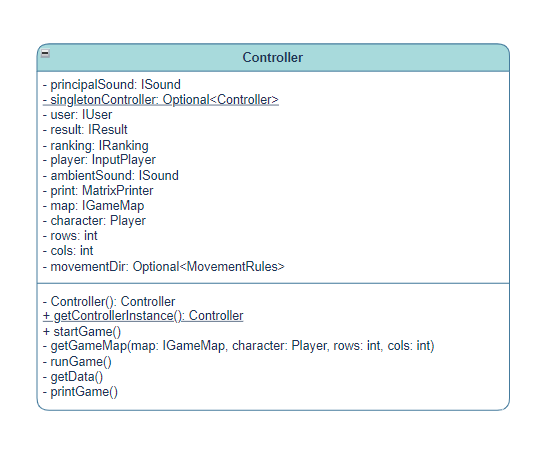
\includegraphics[width=1\textwidth]{controller.png}
            \textbf{Problema}
            \\ \\
            Il Controller è il componente che funge da intermediario tra il modello e la vista in un'architettura MVC. Nel nostro caso il controller ha il compito di aggiornare le informazioni sulla partita a fronte di ogni movimento, modificare i dati del modello come il nome utente, il giocatore selezionato, il livello scelto e infine il risultato parziale che farà parte del ranking.
            \\ \\
            \textbf{Soluzione}
            \\ \\
            Il Controller è formato da una sola classe che si occupa di mettere in comunicazione il modello con la view. Il compito è quindi quello di memorizzare le due istanze e chiamare i rispettivi metodi a fronte di ogni evento generato dall'utente (gli eventi provengono dall'interfaccia grafica). \\
            La classe \textbf{Controller} sta principalmente in ascolto degli input generati dal giocatore. Questi sono dati dalla pressione dei tasti sulla tastiera e dalla scelta dei livelli e personaggi per avviare la partita.\\
            I principali metodi che implementano questa logica sono \verb|getGameMap()|, \verb|runGame()| e \verb|getData()|. Il primo si occupa di ascoltare ciò che viene dai tasti per il movimento del personaggio e inoltrare gli input al modello, il secondo controlla lo stato della partita (che può assumere i valori \verb|GAME_LOST| \verb|GAME_INPROGRESS| e \verb|GAME_WON|) e agisce di conseguenza, mentre l'ultimo serve a ottenere informazioni sul nome utente scelto.\\
            Il Controller si compone delle classi \textbf{User}, \textbf{Result}, \textbf{Ranking}, \textbf{InputPlayer} e \textbf{MatrixPrinter}, mentre imposta una relazione di aggregazione con la classe \textbf{GameMap}
    \newpage
    \subsection{Design della View}
        La View ha il compito di mostrare la partita all'utente e di gestire la raccolta degli input che poi saranno inoltrati al controller; i dati di input si riferiscono principalmente al nome utente, il personaggio scelto, il livello di difficoltà da affrontare e i movimenti rilevati attraverso i tasti W, A, S, D. (rispettivamente, avanti, sinistra, indietro, destra). Si pone, inoltre, il problema di stampare il ranking in caso di vittoria e di mostrare una schermata di game over in caso di sconfitta.\\
        Per la creazione della view abbiamo sviluppato quattro entità principali:
        \begin{itemize}
            \item FileViewer, che mostra all'utente la sua posizione sul ranking quando l'utente non viene ucciso dagli NPC e quindi riesce
            ad uscire dalla mappa, assieme al risultato della partita appena terminata.
            \item MatrixPrinter, che si occupa di stampare la mappa e di aggiornarla a fronte di ogni spostamento dell'utente.
            \item GameOverFrame, che comunica all'utente che ha perso in seguito a un'uccisione per mano di un NPC.
            \item InputPlayer, che mostra la finestra di avvio del gioco tramite cui l'utente riesce a inserire i dati per far cominciare la partita.
        \end{itemize}
        Le entità della view non sono in relazione tra loro, infatti è il controller che si compone della classe MatrixPrinter e InputPlayer e utilizza i metodi delle classi GameOverFrame e FileViewer.
\newpage
\section{Sviluppo}
    \subsection{Testing Automatizzato}
        Per il sistema di entità sono state testate le caratteristiche principali di
        ciascuna delle macro-implementazioni ovvero:
            \begin{itemize}
                \item Per il package \textbf{Characters} è stata testata la classe Fonzie nella sua interezza.
                \item  Per il package \textbf{Elements} sono state testate tutte le classi nella loro interezza
                \item Per il package \textbf{Map} sono stati testati i metodi principali della parte core del modello (presenti nella classe GameMap).
                \item Per il package \textbf{Movement} sono state testate tutte le classi nella loro interezza.
                \item Per il package \textbf{Ranking} è stata testata la classe FileMask nella sua interezza.
                \item Per il package \textbf{Sounds} è stata testata la classe Sound nella sua interezza
            \end{itemize}
        \subsubsection{Characters}
            Per il package Characters ci siamo maggiormente concentrati sul testing di una sola classe per via delle poche differenze con la sua controparte.\\
            La classe è stata testata per tutti i suoi metodi ovvero:
                \begin{itemize}
                    \item Costruttore, abbiamo testato la corretta costruzione della classe con tutti i suoi attributi iniziali, cioè la velocità, le monete e il nome.
                    \item Metodi per gestire le monete del personaggio.
                    \item Metodi per gestire la vita del personaggio.
                    \item Metodi per il corretto funzionamento del salvataggio e la cancellazione delle posizioni, essenziali per l'elemento banana.
                    \item Design Pattern Singleton, abbiamo testato il corretto funzionamento del pattern in questione.
                \end{itemize}
        \subsubsection{Elements}
            Per il package Elements, poiché tutti gli elementi sono essenziali per il modello, li abbiamo testati tutti.
            Seguono i test effettuati per ogni elemento:
                \begin{itemize}
                    \item Box, testato il suo effetto di aggiunta delle monete al giocatore.
                    \item ImmunitySpell, testato il suo effetto di immunità verso gli NPC.
                    \item Banana, testato il suo effetto di far tornare indietro di 5 posizioni il personaggio.
                    \item Bomb, testato il suo effetto di sottrarre monete al giocatore.
                    \item Npc, testato il suo effetto di togliere una vita al personaggio.
                \end{itemize}
        \subsubsection{Gamemap}
            Per il package Gamemap, core del modello, ci siamo concentrati sul testing dei metodi più importanti, ovvero:
                \begin{itemize}
                    \item TestMapGeneration, si occupa di verificare il corretto funzionamento del corrispondente metodo in GameMap per generare dinamicamente la mappa.
                    \item TestRandomElementsGeneration , si occupa del verificare se gli elementi nella mappa sono stati generati correttamente non nella posizione ma nel numero.
                    \item TestMapValidity, si occupa di verificare se a fronte dei precedenti test è una mappa valida per essere giocata ovvero non ci sono collisioni e vi è sempre un percorso per la risoluzione del gioco.
                \end{itemize}
        \subsubsection{Movement}
            Nel testing della macro area denominata Movement ci siamo concentrati sul testing di ogni classe poiché essenziali al modello di cui fanno parte:
                \begin{itemize}
                    \item Movement, testata per tutti i suoi metodi e costruttore, nello specifico è stato testato il corretto funzionamento del movimento in tutte le sue direzioni: su, giù, destra, sinistra, se incontra un muro e i reset del numero di passi del giocatore.
                    \item Position, testato in tutti i suoi metodi.
                \end{itemize}
        \subsubsection{Ranking}
            Nel testing della macro area denominata Ranking ci siamo concentrati sul testing di una sola classe core per denominare il corretto funzionamento della suddetta.
            Testata in tutti i suoi metodi:
                \begin{itemize}
                    \item TestWriteInFile, si occupa di verificare se il file viene popolato correttamente o meno in base alle righe scritte.
                    \item TestSortFile, si occupa di verificare se il sorting del file viene eseguito correttamente o meno controllando il file prima e dopo il sorting e verificando se tutti gli elementi nel file sono ordinati correttamenente
                \end{itemize}
        \subsubsection{Sound}
            Nel testing della macro area denominata Sound ci siamo concentrati nel testing di ogni suono presente nel gioco e del corretto funzionamento della classe preposta che ha i seguenti metodi:
                \begin{itemize}
                    \item PlaySound, ulteriormente testata in tutti i suoni la variante mono, invece la loop (ovvero riproducendo continuamente) una singola volta per semplicità.
                    \item StopSound, testata su un singolo suono per semplicità.
                    \item IsRunning, testata su un singolo suono per semplicità.
                \end{itemize}
    \newpage
    \subsection{Metodologia di Lavoro}
        Strumenti Utilizzati: 
        \begin{itemize}
            \item Git: utilizzato per il versionamento e lo sviluppo cooperativo.
            \item Visual Studio Code: utilizzato come IDE.
            \item GitHub: utilizzato come repository principale.
            \item draw.io: utilizzato per la creazione e la modellazione dell'UML.
            \item Overleaf: utilizzato per la redazione della relazione.
        \end{itemize} 
        Per quanto riguarda la divisione dei compiti, il progetto è stato seguito da tutti i membri in tutte le sue fasi, tuttavia alcuni componenti si sono focalizzati verso aree specifiche del progetto:
        \begin{itemize}
            \item Controller, Viewer e Suoni: Giuseppe Benedetti e Eloi Ricci.
            \item Mappa, Movimento e Posizione: Elia Renzoni e Eloi Ricci.
            \item Personaggi ed Elementi: Annarosa Clemente e Giuseppe Benedetti.
            \item User e Ranking: Elia Renzoni e Giuseppe Benedetti.
            \item Testing: Giuseppe Benedetti.
            \item Relazione: Annarosa Clemente.
        \end{itemize}
    \newpage
    \subsection{Note di Sviluppo}
        Attraverso questo progetto abbiamo appreso e consolidato concetti come \textbf{record} e \textbf{stream}. I primi, introdotti in Java 14 sono utili per la creazione di entità contenenti dati immutabili, mentre gli ultimi ci sono serviti per rendere più moderno e arricchito il codice del nostro progetto. \\
        Oltre a concetti puramente tecnici abbiamo capito l'importanza di standardizzare alcuni aspetti come l'indentazione, l'uso dello stesso editor e lo stile di programmazione.\\
        In particolare ogni membro del gruppo ha imparato i seguenti aspetti:
        \begin{itemize}
            \item Elia Renzoni, ha consolidato l'uso di Git e l'utilizzo di aspetti avanzati di Java come le stream. Inoltre ha imparato a creare il design di un software partendo da idee e concetti, infine ha appreso l'importanza di una buona comunicazione tra i membri del team, per evitare che prevalgano idee senza prima essere concordate e analizzate correttamente. Le principali difficoltà incontrate sono state la gestione del movimento e la creazione della mappa con le limitazioni sul numero di ostacoli e sulle mura.
            \item Annarosa Clemente...
            \item Giuseppe Benedetti, ha consolidato le competenze tecniche come: l'uso di git, dell'IDE VSCodium, uso del LaTeX per le relazioni, aspetti avanzati di Java come: le stream, i record, le operazioni su file, il suono, la grafica tramite JavaFX e i test automatizzati junit.\\
            Inoltre ha imparato l'importanza di una buona comunicazione con i membri del team, che comprende, l'organizzazione del lavoro con il metodo top-down derivato dalla modellazione del design di un software, l'importanza di eseguire al meglio, in tempo, i propri compiti e non fare di testa propria, ma avere uno spirito pronto al confronto ascoltando gli altri membri del team.  
            \item Eloi Ricci, ho consolidato l'uso di ChatGPT e git push --force.
        \end{itemize}
\end{document}
